\documentclass[a4paper, 12pt, notitlepage]{article}
\usepackage[letterpaper,margin=1in,marginparwidth=1.75cm]{geometry}
\usepackage{graphicx, booktabs, tikz, csquotes, subfig, dcolumn}
\usepackage[font=small,labelfont=bf]{caption}
% \usepackage[markers,figuresonly,nolists]{endfloat}
\usepackage[natbibapa]{apacite}
\usepackage[colorlinks = TRUE, allcolors = blue]{hyperref}
\usepackage[section]{placeins}

\usepackage{setspace}
\setstretch{1.25}

\renewcommand*\rmdefault{ppl}

\title{\Large Online appendix for\\Violence, co-optation, and postwar voting in Guatemala}
\author{}%Francisco Villamil}
\date{}

% Section numbering
\renewcommand{\thesection}{\Alph{section}}

% Table numbering
\renewcommand{\thetable}{A\arabic{table}}

% Table numbering
\renewcommand{\thefigure}{A\arabic{figure}}

\begin{document}

\maketitle

\tableofcontents


\clearpage
\section{Territorial changes in municipalities}

A `minimum denomination' of municipalities was built, by joining together those municipalities where changes took place, which consisted mainly of splits.
Thus, if a new municipality was formed out of a bigger one, the two are merged again in the dataset, so as to ensure compatibility between data sources across time.
In particular, the dataset contains observations that range from 1973 to 2015, during which time there has been 15 territorial changes at the local level.
Although one variable goes further back in time, namely rebel activity before 1978, only two territorial changes took place before that date: the formation of Melchor de Mencos (1962) and Poptún (1966).%, both in the department of Petén.
Given that no rebel activity was recorded in the whole territory of Petén before 1971, these two changes were not implemented.
Table \ref{tab-app:muni} below shows the municipalities that were formed, along with the data and the parent municipality they are merged to in the dataset.

\begin{table}[!htbp] \centering
  \caption{Municipality changes in Guatemala, 1973--2015}
  \label{tab-app:muni}
  \small
  \begin{tabular}{cccc}
  \\[-1.8ex]\hline
  \hline \\[-1.8ex]
  \\[-1.8ex]
  Department      & New municipality                & Date      & Parent municipality \\
  \hline \\[-1.8ex]
  Alta Verapaz    & Fray Bartolomé de las Casas     & 1980      & Santa María Cahabón \\
  Alta Verapaz    &                    La Tinta     & 1999      &              Panzás \\
  Alta Verapaz    &                     Raxruhá     & 2008      &              Chisec \\
  Escuintla       &            Nueva Concepción     & 1974      &           Tiquisate \\
  Escuintla       &                    Sipacate     & 2015      &           La Gomera \\
  Huehuetenango   &              Unión Cantinil     & 2005      &            Chiantla \\
  Peten           &                     El Chal     & 2014      &             Dolores \\
  Peten           &                  Las Cruces     & 2011      &         La Libertad \\
  Quiche          &                    Chicamán     & 1984      &            Uspantán \\
  Quiche          &                       Ixcán     & 1985      &            Uspantán \\
  Quiche          &                    Pachalúm     & 1986      &             Joyabaj \\
  San Marcos      &                   La Blanca     & 2014      &                Ocós \\
  Suchitepequez   &         San Jose La Maquiná     & 2014      &         Cuyotenango \\
  Zacapa          &                   San Jorge     & 2014      &              Zacapa \\
  \hline
  \hline \\[-1.8ex]
  \end{tabular}
\end{table}

\clearpage
\section{Accessibility and violence against civilians}

Table \ref{tab-gt:corr_vio_state} shows the results of linear models explaining wartime violence by the state.
Models in the first two columns run the analyses for the whole sample, including department fixed effects in column 2.
Columns 3 and 4 show equivalent models but restricting the sample to only the most affected departments.

State violence does not have any relevant relationship with the two proxy variables used as interactions.
If anything, it has a positive relationship with the distance to the Pan-American Highway in column 2.
Regarding the other variables, state violence is mainly explained by the share of indigenous population in each municipality and by its size.
When limiting the sample to the most affected departments and including fixed effects, the share of indigenous population stops being significant.

Table \ref{tab-gt:corr_vio_rebel} shows the results for models equivalent to the previous ones but using rebel violence as the dependent variable.
Although patterns of rebel violence should not be as relevant to the argument advanced here, it is important to check whether any of the two accessibility proxies is related to local wartime activity.

Again, none of the accessibility proxies shows any relationship to rebel violence.
Rebel violence is also poorly explained by the rest of the variables.
Perhaps because of the relatively low incidence of violence by the rebels, no robust relationship is found.

The results show that the two accessibility variables used as proxies for the level of exposure to prewar mobilization are not related to the intensity of the conflict in each municipality.

\input{../../../../dissertation/empirics/guatemala/table_correlates_state_vio.tex} %tab-gt:corr_vio_state

\input{../../../../dissertation/empirics/guatemala/table_correlates_rebel_vio.tex} %tab-gt:corr_vio_rebel

\clearpage
\section{Additional results}

\subsection{Using only CEH data for violence}

Tables \ref{tab-gt:int_roads_ceh} and \ref{tab-gt:int_panam_ceh} replicate the main results using only CEH data to measure wartime violence.

\subsection{Combining electoral share by FRG and PP}

Table \ref{tab-gt:full_dcha} shows the results of the main models using as the dependent variable the combined electoral share of the FRG and the PP.
Figures \ref{fig-app:pp_fulldcha_roads} and \ref{fig-app:pp_fulldcha_panam} show the results visually.

\subsection{Cross-sectional results by election}

Tables \ref{tab-gt-app:base_URNGyrs} and \ref{tab-gt-app:base_FRGyrs} show results of running the base model without interactions, using a cross-sectional data for each election since 1999.
Tables \ref{tab-gt-app:panam_URNGyrs}, \ref{tab-gt-app:roads_URNGyrs}, \ref{tab-gt-app:panam_FRGyrs}, and \ref{tab-gt-app:roads_FRGyrs} do the same but including the interaction with the accessibility proxies.
Figures \ref{fig-app:pp_urng_panam_yrs}, \ref{fig-app:pp_urng_roads_yrs}, \ref{fig-app:pp_frg_panam_yrs}, and \ref{fig-app:pp_frg_roads_yrs} show these results visually.

% Table \ref{tab-gt-app:base_URNGyrs} shows results of running the base model without interactions for the voting share of URNG using a cross-sectional data for each election since 1999.
% Table \ref{tab-gt-app:base_FRGyrs} shows the same models for the FRG.
% In the case of URNG, state violence shows a positive effect in the first elections in 1999, but this effect disappears after that year.
% State violence does not play any meaningful effect in explaining local-level FRG vote in any election, and neither do the rest of the variables.
%
% Models in table \ref{tab-gt-app:panam_URNGyrs} again analyze URNG vote in each of the election years separately, in this case including the interaction with the distance to the Pan-American Highway.
% Table \ref{tab-gt-app:roads_URNGyrs} does the same, but including the interaction with the share of non-paved roads.
% Figures \ref{fig-app:pp_urng_panam_yrs} and \ref{fig-app:pp_urng_roads_yrs} show these results visually.
%
% Tables \ref{tab-gt-app:panam_FRGyrs} and \ref{tab-gt-app:roads_FRGyrs} replicate these previous analyses for FRG vote, including the interaction with distance to the Pan-American Highway and with the share of non-paved roads, respectively.
% Again, results are shown visually in figures \ref{fig-app:pp_frg_panam_yrs} and \ref{fig-app:pp_frg_roads_yrs} for better interpretation.


\input{../../../../dissertation/empirics/guatemala/table_roads_nonpaved_ceh.tex}
\input{../../../../dissertation/empirics/guatemala/table_dist_panam_ceh.tex}

\input{../../../../dissertation/empirics/guatemala/table_full_dcha.tex}

\begin{figure*}[htb!]
  \centering
    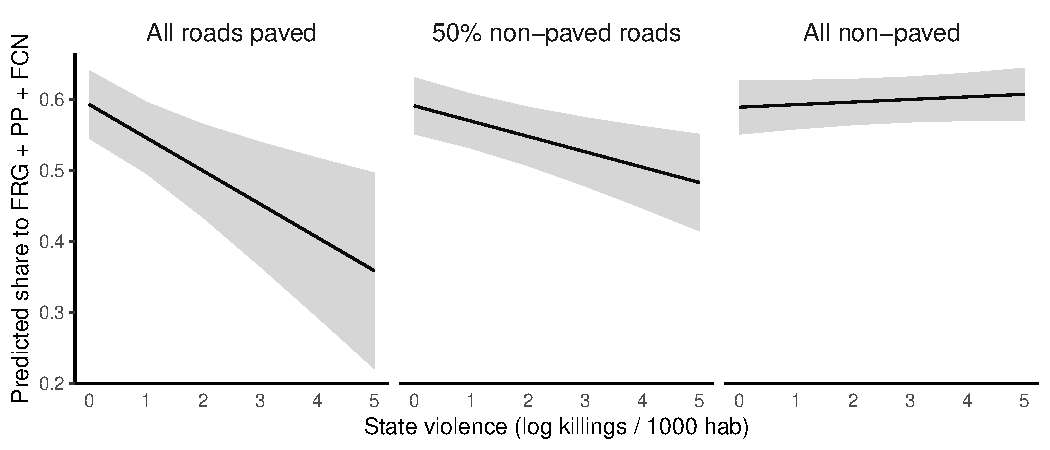
\includegraphics[width = 0.7\textwidth]{../../../../dissertation/empirics/guatemala/pp_fulldcha_roads}

  \caption{Wartime state violence and FRG/PP share depending on prewar political mobilization (proxied by \% non-paved roads)} \label{fig-app:pp_fulldcha_roads}

\end{figure*}

\begin{figure*}[htb!]
  \centering
    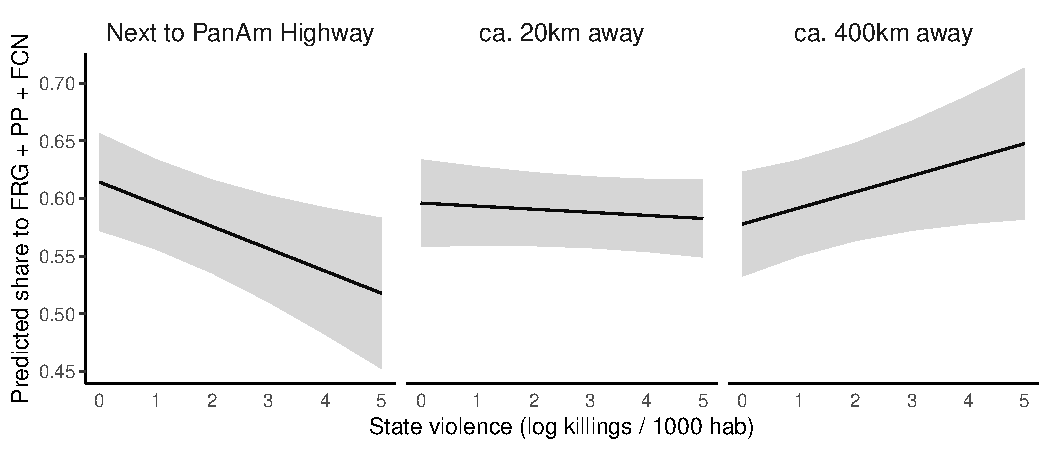
\includegraphics[width = 0.7\textwidth]{../../../../dissertation/empirics/guatemala/pp_fulldcha_panam}

  \caption{Wartime state violence and FRG/PP share depending on prewar political mobilization (proxied by distance to Pan-American Highway)} \label{fig-app:pp_fulldcha_panam}

\end{figure*}

\input{../../../../dissertation/empirics/guatemala/table_app_base_URNG_yrs.tex}
\input{../../../../dissertation/empirics/guatemala/table_app_base_FRG_yrs.tex}

\input{../../../../dissertation/empirics/guatemala/table_app_URNG_panam_yrs.tex}
\input{../../../../dissertation/empirics/guatemala/table_app_URNG_roads_yrs.tex}

\begin{figure*}[htb!]
  \centering
    \includegraphics[width = \textwidth]{../../../../dissertation/empirics/guatemala/pp_urng_panam_yrs}

  \caption{Wartime state violence and URNG share depending on prewar political mobilization (proxied by distance to Pan-American Highway)} \label{fig-app:pp_urng_panam_yrs}

\end{figure*}

\begin{figure*}[htb!]
  \centering
    \includegraphics[width = \textwidth]{../../../../dissertation/empirics/guatemala/pp_urng_roads_yrs}

  \caption{Wartime state violence and URNG share depending on prewar political mobilization (proxied by \% non-paved roads)} \label{fig-app:pp_urng_roads_yrs}

\end{figure*}

\input{../../../../dissertation/empirics/guatemala/table_app_FRG_panam_yrs.tex}
\input{../../../../dissertation/empirics/guatemala/table_app_FRG_roads_yrs.tex}

\begin{figure*}[htb!]
  \centering
    \includegraphics[width = 0.7\textwidth]{../../../../dissertation/empirics/guatemala/pp_frg_panam_yrs}

  \caption{Wartime state violence and FRG share depending on prewar political mobilization (proxied by distance to Pan-American Highway)} \label{fig-app:pp_frg_panam_yrs}

\end{figure*}

\begin{figure*}[htb!]
  \centering
    \includegraphics[width = 0.7\textwidth]{../../../../dissertation/empirics/guatemala/pp_frg_roads_yrs}

  \caption{Wartime state violence and FRG share depending on prewar political mobilization (proxied by \% non-paved roads)} \label{fig-app:pp_frg_roads_yrs}

\end{figure*}

\end{document}
